\documentclass[12pt,compress]{beamer}
\usepackage{ifthen,ulem}

\title{Track-based Alignment for the \\ Muon Chambers \\ (just starting!)}
\author{Jim Pivarski}
\institute{Texas A\&M University}
\date{6 October, 2006}

\setbeamertemplate{navigation symbols}{}
\setbeamertemplate{headline}{\includegraphics[height=1 cm]{../cmslogo} \hspace{0.1 cm} \includegraphics[height=1 cm]{../tamulogo} \hfill
\begin{minipage}{9 cm}
\vspace{-0.75 cm} \small
\begin{center}
\ifthenelse{\equal{\insertpagenumber}{1}}{}{\insertsection}
\end{center}
\end{minipage} \hfill
\begin{minipage}{1 cm}
\vspace{-0.75 cm} \small
\begin{center}
\ifthenelse{\equal{\insertpagenumber}{1}}{}{\insertpagenumber/\pageref{numpages}}
\end{center}
\end{minipage}}

\xdefinecolor{verylightgray}{rgb}{0.95,0.95,0.95}
\beamertemplateshadingbackground{verylightgray}{white}

\begin{document}
\frame{\titlepage}
\section*{Track-based Muon Alignment --- Jim Pivarski}

\begin{frame}
\frametitle{What this talk is NOT}

I don't intend to present an overview of track-based alignment.

\vfill
Here are some references for that

\vspace{0.5 cm}
\begin{minipage}{\linewidth}
\scriptsize
\begin{itemize}
  \item CMS NOTE 2006/016: {\bf Muon System alignment with tracks}
  \item CMS NOTE 2006/017: Influence of Misalignment Scenarios on Muon \\ \hspace{3.5 cm} Reconstruction
\end{itemize}

\begin{itemize}
  \item CMS NOTE 2006/011: Software Alignment of the CMS Tracker using \\ \hspace{3.5 cm} {\bf MILLEPEDE II}
  \item CMS NOTE 2006/018: The {\bf HIP Algorithm} for Track Based Alignment and its \\ \hspace{3.5 cm} Application to the CMS Pixel Detector
  \item CMS NOTE 2006/022: A {\bf Kalman Filter} for Track-based Alignment
\end{itemize}
\end{minipage}

\vfill
We (Texas A\&M) are newcomers to this project.
\end{frame}

\begin{frame}
\frametitle{This talk is about our plans for getting involved}
\begin{description}\setlength{\itemsep}{1 cm}
  \item[Objective:] develop a track-based muon alignment package for CMSSW
  \item[Method:] extend existing tracker alignment tools to muon detector
  \item[Short-term (this talk):] get up to speed on muon software infrastructure
\end{description}
\end{frame}

\begin{frame}
\frametitle{Strategy}
\begin{enumerate}\setlength{\itemsep}{0.5 cm}
  \item Obtain a sample with DT \& CSC hits and standalone or global muon tracks \textcolor{red}{$\surd$}
  \item Plot global positions of DT \& CSC hits \textcolor{red}{$\surd$}
  \item Apply a misalignment and observe a shift in hit positions
  \item Start writing/porting/linking to an alignment algorithm
  \item Obtain large, realistic $Z \to \mu\mu$ and $W \to \mu\nu$ samples to study performance
\end{enumerate}
\end{frame}

\begin{frame}
\frametitle{Step 1 (get a sample): DONE}
Found a $H \to ZZ \to \mu\mu\mu\mu$ physics validation sample with muon hits and global fits
\begin{quote}
\rm \scriptsize https://twiki.cern.ch/twiki/bin/view/CMS/RelValSamples
\end{quote}

We filtered out all branches except reco::Tracks, reco::TrackExtras, and
TrackingRecHits, to make it like AlCaRECO.

\vfill
\sout{(The LPC $Z \to \mu\mu$ samples have no muon hits.)}

\it
\textcolor{blue}{On Wednesday, Sergei Gleyzer pointed me to CMSSW\_1\_0\_1 samples. (I haven't checked them yet.)}

\vfill
\textcolor{blue}{Official AlCaRECO with muons is coming in CMSSW\_1\_0\_4.}
\end{frame}

\begin{frame}
\frametitle{Step 2 (plot global hit positions): DONE}
\begin{columns}[c]

\column{0.4\linewidth}
\begin{minipage}{\linewidth}
\begin{raggedright}
\scriptsize
extracted
ESHandle$<$DTGeometry$>$ and
ESHandle$<$CSCGeometry$>$
from MuonGeometryRecord to transform localCoordinates into
globalCoordinates
\end{raggedright}
\end{minipage}

\column{0.55\linewidth}
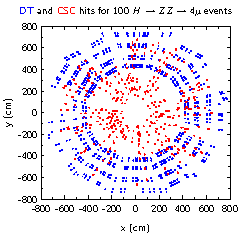
\includegraphics[width=\linewidth]{rphi_hits}
\end{columns}
\end{frame}

\begin{frame}
\frametitle{Step 2 (plot global hit positions): DONE}
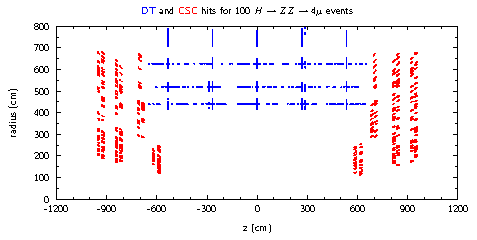
\includegraphics[width=\linewidth]{rz_hits}
\end{frame}

\begin{frame}
\frametitle{Step 3 (apply a misalignment): \textcolor{red}{not working}}
I tried to apply it, but nothing moves (CMSSW\_1\_0\_1)

\vfill
\begin{description}
  \item[Perfect Alignment]
\end{description}

\begin{minipage}{\linewidth}
  \begin{flushleft}
    \scriptsize
    include "Geometry/CMSCommonData/data/CMSIdealGeometryXML.cfi" \\
    include "Geometry/DTGeometry/data/dtGeometry.cfi" \\
    include "Geometry/CSCGeometry/data/cscGeometry.cfi"
  \end{flushleft}
\end{minipage}

\begin{description}
  \item[Misaligned]
\end{description}

\begin{minipage}{\linewidth}
  \begin{flushleft}
    \scriptsize
    include "Geometry/CMSCommonData/data/CMSIdealGeometryXML.cfi" \\
    include "Alignment/MuonAlignment/data/Scenarios.cff" \\
    es\_module MisalignedMuon = MisalignedMuonESProducer \{using \\
    \hfill MuonExampleScenario\}
  \end{flushleft}
\end{minipage}

\hfill {\scriptsize also tried MuonSurveyOnlyScenario\ldots}

\vfill (Other combinations of commenting things out didn't cmsRun.  I
need to talk to Andre Sznajder, the author.)
\end{frame}

\begin{frame}
\frametitle{Steps 4 and 5 (use framework/realistic dataset)}
Oliver Buchmueller (Friday):
\begin{quote}
Andre Sznajder and Frederic Ronga have just a few days ago committed
in 1\_0\_2 (and 1\_0\_3) the full muon alignment geometry interface to
the DB.
\end{quote}

\vfill We also got in touch with Francisco Matorras, who is working on
a similar project in Santander, Spain.  His group has calculated
residuals and written to the database, two things we'll need to do also.

\vfill
We'll get together and figure out how to collaborate.
\end{frame}

\begin{frame}
\frametitle{Summary}
We're past the CMSSW start-up issues, ready for muon/alignment specifics.

\vfill
Now we only need to
\begin{enumerate}[\alph{enumi}) ]
\item misalign the detector (MisalignedMuonESProducer),
\item move it back (AlignableMuonModifier), and
\item write an algorithm to do so automatically (CMS~NOTES/talk to
Francisco/look at tracker implementation).
\end{enumerate}
\label{numpages}
\end{frame}

\end{document}
